\chapter{Introduction}
\label{ch:introduction}

Ever since the creation of the first computers, humans started to wonder whether such complex machines could one day be able to think. Already in the 20th century, computer scientist Alan Turing, who by many is considered to be the main progenitor of computer science, designed the \textit{Imitation Game}, an experiment devoted to test whether a machine can exhibit intelligent behaviors. While purely theoretical, as well as philosophical, his work opened the door to many questions that throughout the years would have defined the field of Artificial Intelligence (AI), a multidisciplinary field that aims to create computer programs that are able to mimic, at least in part, the cognitive abilities underlying human intelligence. In the attempt of answering Turing's everlasting question \textcolor{RoyalBlue}{\textit{Can machines think?}}, part of the AI community started to consider an equally challenging and foundamental question: \textcolor{RoyalBlue}{\textit{Can machines learn?}}. This question is nowadays being tackled by researchers working at the intersection of computer science, probability, statistics and even information theory and psychology, which all fall under the research field that is denoted as machine learning.

The question \textit{Can machines learn?} might only at first sight appear to be simple and straightforward to answer, as in reality it actually forces us to define two very important concepts. First, while it is true that the term machine has to relate to computer programs, it is equally true that it gives little insight about the computational nature of such programs, which in practice can come in very different flavours as they are typically built on top of a wide range of mathematical models. Second, it also requires us to consider what it means for a computer program to \textit{learn} and how such an ability, which by many cognitive scientists is considered to be one of the main intellectual feats underlying intelligence, is related to computer science, a discipline that at first sight might have little in common with research fields that study the human brain. 

\section{Machine Learning}

According to \citet{mitchell1997machine} a computer program, is said to \textcolor{RoyalBlue}{learn} if it manages to improve its performance on a certain task through experience.
Examples of potential tasks might be the recognition of digits in images \cite{lecun1994mnist}, mastering a certain boardgame \cite{silver2017mastering}, or even the ability of predicting the outcome of a clinical trial \cite{zhao2011reinforcement}. While tasks can come in numerous flavours and can differ across eachother in terms of complexity, the way these are usually tackled by a learning algorithm can be divided into three different paradigms. While two of these three learning scenarios will be covered in depth in the first part of this dissertation we still briefly describe them hereafter.

\begin{enumerate}
	\item \textcolor{RoyalBlue}{Supervised Learning}: this instance of machine learning is characterized by problems where there is an input space $\mathcal{X}$ and an output space $\mathcal{Y}$ and the goal is to learn a mapping $f$ from $\mathcal{X}$ to $\mathcal{Y}$. The computer program can learn this mapping thanks to some input-output pairs that are i.i.d. drawn from the joint probability distribution $P(X,Y)$ and that can be observed throughout the learning process. Broadly speaking, the more the program observes these input-output pairs, the more experienced it gets and therefore the more accurate its mapping function becomes.  
	\item \textcolor{RoyalBlue}{Unsupervised Learning}: in this scenario the learning algorithm does not have access to any output values drawn from $P(X,Y)$ and therefore cannot rely on them throughout the learning process. As a result the aforementioned mapping function $f$ cannot be learned. Instead, unsupervised learning algorithms aim at discovering occurring patterns within the input samples they observe.  
	\item \textcolor{RoyalBlue}{Reinforcement Learning}: is a branch of machine learning where an agent has to learn how to interact with its surroundings, typically defined as the environment. Thanks to an interactive learning procedure, known as the agent-environment loop, the agent's goal is that of learning an optimal policy $\pi^{*}$, which allows it to maximize a certain reward signal over time. Differently from the two learning paradigms mentioned above, reinforcement learning is a much more dynamic and uncertain learning scenario, which builds on top of ideas stemming from a large variety of disciplines ranging from mathematical optimization to cognitive psychology.   
\end{enumerate}


Several learning algorithms able of dealing with the aforementioned learning scenarios exist, however, the last years have witnessed the developement of many successfull applications that are based on artificial neural networks. Among the different types of possible artificial neural networks, strong potential has been exhibited in all three machine learning areas by \textcolor{RoyalBlue}{Convolutional Neural Networks} (CNNs), a class of techniques that is particularly well suited for dealing with high-dimensional and spatially organized inputs such as images. Computer programs based on CNNs are to this date the state of the art when it comes to a large variety of machine learning tasks. In fact, CNNs are nowadays able of successfully dealing with supervised learning problems that involve the classification of natural images (see Figure \ref{fig:dogo}), and even to learn how to play popular arcade videogames without any supervision (see Figure \ref{fig:dqn_example}).

\begin{figure}[ht!]
\centering
  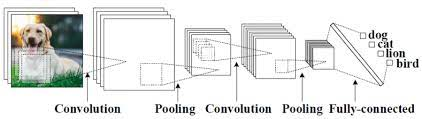
\includegraphics[width=10cm]{./Images/Chapter00/dogo}
  \caption{An example of a Convolutional Neural Network that gets trained for solving a supervised learning problem, namely correctly classifying the animal depicted in the image as a dog. The different components of this network will be explained in detail in Chapter \ref{ch:supervised_learning} of this dissertation. Image taken from \cite{dogoimage}.}
  \label{fig:dogo}
\end{figure}

\begin{figure}[ht!]
\centering
  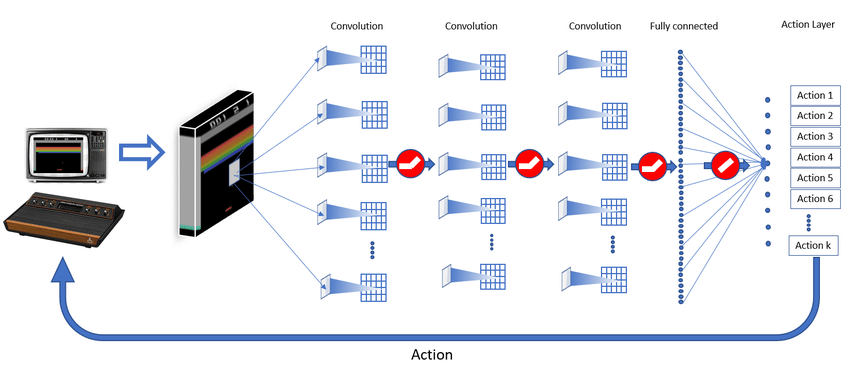
\includegraphics[width=10cm]{./Images/Chapter00/dqn}
  \caption{An example of a Convolutional Neural Network trained for solving a reinforcement learning problem, namely learning how to play the arcade Atari game of \texttt{Breakout}. The way the network achieves this task will be presented in detail in Chapter \ref{ch:reinforcement_learning}. Image courtesy of \citet{patel2019improved}.}
  \label{fig:dqn_example}
\end{figure}




\section{Objectives and Research Questions}

The typical machine learning training scenario assumes that when the learning process begins, a computer program starts solving a certain task \textcolor{RoyalBlue}{\textit{tabula rasa}}. Going back to the examples presented in Fig. \ref{fig:dogo} and Fig. \ref{fig:dqn_example}, this corresponds to a situation where a CNN has either never dealt with the supervised learning problem of natural image classification, or has never learned how to play any Atari videogame before facing the \texttt{Breakout} game depicted in the image. While overall CNNs are able of successfully learning how to solve a certain machine learning problem from scratch, there can however be certain situations
where learning from scratch can result in sub-optimal performance or even prevent a network from  learning at all. Based on this potential limitation, the work presented in this dissertation aims at exploring whether this family of neural networks can get transferred and trained across different tasks, and aims to identify which sort of benefits can arise from tackling several machine learning problems with CNNs that instead of being trained from scratch have already been pre-trained on related tasks in the past. Therefore, driven by the following general research question:
\begin{center}
	\textit{Can convolutional neural networks be transferred and trained across different source and target domains? if so, which target domains could be of interest for investigating their transfer learning properties?}	
\end{center}    
we aim at better charactering the transfer learning properties of CNNs, and investigate whether this family of machine learning models can get transferred both in a supervised learning scenario as well as in a reinforcement learning one. We will help answer this research question by addressing three, arguably more specific, research questions which are:
\begin{enumerate}
	\item \textit{What Transfer Learning training strategy should be adopted to maximize the performance of pre-trained networks?}

	\item \textit{Can Transfer Learning be a valuable tool for better understanding convolutional neural networks?}
	
	\item \textit{Do different machine learning paradigms result in convolutional neural networks with different transfer learning properties?}
\end{enumerate}


\section{Outline of the Dissertation}


As mentioned earlier, all research questions will be studied both from a supervised learning perspective as well as from a reinforcement learning one, while at the same time leaving a transfer learning study for the unsupervised learning scenario as future work. It naturally follows that after having introduced these learning paradigms in Chapters \ref{ch:supervised_learning}, \ref{ch:reinforcement_learning} and \ref{ch:transfer_learning}, the rest of this dissertation will be divided into two more parts: Part II, including Chapters \ref{ch:tl_natural_to_non_natural}, \ref{ch:minerva} and \ref{ch:tl_lth}, which will focus on studying the transfer learning potential of CNNs within supervised learning; and Part III, made of Chapters \ref{ch:dqv_family_of_algorithms}, \ref{ch:dqn_transfer} and \ref{ch:upside_down_rl}, which will focus on the reinforcement learning scenario instead. More specifically, in Part II we will focus our supervised transfer learning analysis on domains that are not defined within the realm of natural images and that see instead CNNs applied in the areas of digital heritage (Chapters \ref{ch:tl_natural_to_non_natural}, \ref{ch:minerva} and \ref{ch:tl_lth}) and digital pathology (Chapter \ref{ch:tl_lth}). Here we will be considering computer vision tasks ranging from image classification to object detection. In Part III, our transfer learning studies will consider the domain of model-free deep reinforcement learning, a research area that aims to solve optimal control problems with convolutional neural networks that need to serve as value function approximators as well as feature extractors. Here we will see how this task differs from the aforementioned computer vision problems and how it affects the overall transfer learning properties of CNNs. 


\section{Publications}

The aforementioned research questions will be answered thanks to the work that has been presented in several peer-reviewed publications. These contributions, together with the role they play throughout this dissertation, are presented in chronological order hereafter:

\begin{remark}{Main Publications}
\begin{itemize}
	\item \citet{sabatelli2018deep} \textit{"Deep transfer learning for art classification problems."} Proceedings of the European Conference on Computer Vision (ECCV) Workshops, 2018.
	\\ This publication will be mainly reviewed in Chapter \ref{ch:tl_natural_to_non_natural}, and will be of interest in Chapters \ref{ch:minerva}, \ref{ch:tl_lth} and \ref{ch:dqn_transfer}.

	\item \citet{sabatelli2018deepqv} \textit{Deep Quality Value (DQV) Learning."} Advances in Neural Information Processing Systems (NeurIPS), Deep Reinforcement Learning Workshop, 2018.
	\\ This publication is of interest in Chapter \ref{ch:dqv_family_of_algorithms} and \ref{ch:dqn_transfer}.

	\item \citet{sabatelli2019approximating}  \textit{"Approximating two value functions instead of one: towards characterizing a new family of Deep Reinforcement Learning algorithms"} Advances in Neural Information Processing Systems (NeurIPS), Deep Reinforcement Learning Workshop, 2019. \\
	This publication is of interest in Chapter \ref{ch:dqv_family_of_algorithms}.
	
	\item \citet{sabatelli2020deep} \textit{"The deep quality-value family of deep reinforcement learning algorithms"} Proceedings of the International Joint Conference on Neural Networks (IJCNN). IEEE, 2020.
	\\ This is the main publication underlying Chapter \ref{ch:dqv_family_of_algorithms}, which will also be of interest in Chapter \ref{ch:dqn_transfer}.

	\item \citet{sabatelli2020transferability} \textit{"On the transferability of winning tickets in non-natural image datasets.} Proceedings of the 16th International Joint Conference on Computer Vision, Imaging and Computer Graphics Theory and Applications (VISAPP), 2021.
	\\ This work was also presented at the first edition of the Sparsity in Neural Networks (SNN) Workshop 2021.
	\\ Chapter \ref{ch:tl_lth} is based on this publication.

	\item \citet{sabatelli2021advances} \textit{"Advances in Digital Music Iconography: Benchmarking the detection of musical instruments in unrestricted, non-photorealistic images from the artistic domain."} DHQ: Digital Humanities Quarterly 15.1 2021.
	\\ Chapter \ref{ch:minerva} extends this publication.

	\item \citet{sabatelli2021transferability} \textit{"On the Transferability of Deep-Q Networks."} Advances in Neural Information Processing Systems (NeurIPS), Deep Reinforcement Learning Workshop, 2021. \\
	Chapter \ref{ch:dqn_transfer} is based on this publication.
 
\end{itemize}
\end{remark}

Throughout the Ph.D. several other peer-reviewed papers have been published, however these are not directly presented in this thesis as they are either the result of external collaborations, or have served for reporting preliminary results of ongoing research:

\begin{takeaway}{Additional Publications}
\begin{itemize}
	\item \citet{leroy21qvmix} \textit{"QVMix and QVMix-Max: Extending the Deep Quality-Value Family of Algorithms to Cooperative Multi-Agent Reinforcement Learning."} Proceedings of the AAAI-21 Workshop on Reinforcement Learning in Games, 2021. 
	\item \citet{hammond2020forest} \textit{"Forest Fire Control with Learning from Demonstration and Reinforcement Learning".} Proceedings of the International Joint Conference on Neural Networks (IJCNN). IEEE, 2020.
	\item \citet{banartransfer} \textit{"Transfer Learning with Style Transfer between the Photorealistic and Artistic Domain."} IS\&T International Symposium on Electronic Imaging. Computer Vision and Image Analysis of Art, 2021.
	\item \citet{sasso2021fractional} \textit{"Fractional Transfer Learning for Deep Model-Based Reinforcement Learning."} \\ ArXiv preprint arXiv:2108.06526. 

\end{itemize}
\end{takeaway}
